% Options for packages loaded elsewhere
\PassOptionsToPackage{unicode}{hyperref}
\PassOptionsToPackage{hyphens}{url}
%
\documentclass[
]{article}
\usepackage{lmodern}
\usepackage{amsmath}
\usepackage{ifxetex,ifluatex}
\ifnum 0\ifxetex 1\fi\ifluatex 1\fi=0 % if pdftex
  \usepackage[T1]{fontenc}
  \usepackage[utf8]{inputenc}
  \usepackage{textcomp} % provide euro and other symbols
  \usepackage{amssymb}
\else % if luatex or xetex
  \usepackage{unicode-math}
  \defaultfontfeatures{Scale=MatchLowercase}
  \defaultfontfeatures[\rmfamily]{Ligatures=TeX,Scale=1}
\fi
% Use upquote if available, for straight quotes in verbatim environments
\IfFileExists{upquote.sty}{\usepackage{upquote}}{}
\IfFileExists{microtype.sty}{% use microtype if available
  \usepackage[]{microtype}
  \UseMicrotypeSet[protrusion]{basicmath} % disable protrusion for tt fonts
}{}
\makeatletter
\@ifundefined{KOMAClassName}{% if non-KOMA class
  \IfFileExists{parskip.sty}{%
    \usepackage{parskip}
  }{% else
    \setlength{\parindent}{0pt}
    \setlength{\parskip}{6pt plus 2pt minus 1pt}}
}{% if KOMA class
  \KOMAoptions{parskip=half}}
\makeatother
\usepackage{xcolor}
\IfFileExists{xurl.sty}{\usepackage{xurl}}{} % add URL line breaks if available
\IfFileExists{bookmark.sty}{\usepackage{bookmark}}{\usepackage{hyperref}}
\hypersetup{
  hidelinks,
  pdfcreator={LaTeX via pandoc}}
\urlstyle{same} % disable monospaced font for URLs
\usepackage[left = 20mm, right = 20mm, top = 10mm, bottom =
45mm]{geometry}
\usepackage{longtable,booktabs}
\usepackage{calc} % for calculating minipage widths
% Correct order of tables after \paragraph or \subparagraph
\usepackage{etoolbox}
\makeatletter
\patchcmd\longtable{\par}{\if@noskipsec\mbox{}\fi\par}{}{}
\makeatother
% Allow footnotes in longtable head/foot
\IfFileExists{footnotehyper.sty}{\usepackage{footnotehyper}}{\usepackage{footnote}}
\makesavenoteenv{longtable}
\usepackage{graphicx}
\makeatletter
\def\maxwidth{\ifdim\Gin@nat@width>\linewidth\linewidth\else\Gin@nat@width\fi}
\def\maxheight{\ifdim\Gin@nat@height>\textheight\textheight\else\Gin@nat@height\fi}
\makeatother
% Scale images if necessary, so that they will not overflow the page
% margins by default, and it is still possible to overwrite the defaults
% using explicit options in \includegraphics[width, height, ...]{}
\setkeys{Gin}{width=\maxwidth,height=\maxheight,keepaspectratio}
% Set default figure placement to htbp
\makeatletter
\def\fps@figure{htbp}
\makeatother
\setlength{\emergencystretch}{3em} % prevent overfull lines
\providecommand{\tightlist}{%
  \setlength{\itemsep}{0pt}\setlength{\parskip}{0pt}}
\setcounter{secnumdepth}{-\maxdimen} % remove section numbering
\usepackage{fancyhdr, graphicx, eurosym, booktabs, xcolor, lastpage} \pagestyle{fancy} \fancyhf{} \addtolength{\headheight}{2.5cm} \fancyheadoffset{10mm} \lhead{\IfFileExists{logo.png}{\includegraphics[height = 2cm]{logo.png}}} \lfoot{Page \thepage~of~\pageref{LastPage}} \fancypagestyle{plain}{\pagestyle{fancy}} \renewcommand{\headrulewidth}{0pt} \setlength{\headsep}{12mm} \usepackage{titling} \usepackage{booktabs} \usepackage{multicol} \setlength{\belowcaptionskip}{0pt plus 1pt minus 1pt}
\ifluatex
  \usepackage{selnolig}  % disable illegal ligatures
\fi

\author{}
\date{\vspace{-2.5em}}

\begin{document}

\(~\)

\vspace{5ex}
\begin{center}\textsc{\huge Calibration Certificate Information}\end{center}
\vspace{8ex}

\textbf{\Large Calibrating Laboratory}\newline \textbf{Adress}
\vspace{4ex}

\hypertarget{certificate-number-4637}{%
\subsection{\texorpdfstring{Certificate number:
\textbf{4637}}{Certificate number: 4637}}\label{certificate-number-4637}}

\(\hrulefill\)

\(~\)

\begin{tabular}{@{$\qquad\qquad$}rp{0.7\linewidth}}
 \textbf{\large Object to calibrate:}&\textbf{\large Non Automatic Weighing Instrument (NAWI)}\\[3ex]
 \textbf{Identification:}&Balanza Mettler Toledo XPE 205\\
 \textbf{Serial:}&B743848411 / AF-07090\\
 \textbf{Calibration date:}&2020-07-16\\
 \textbf{Calibration place:}&Bogotá - Colombia.  Avenida Carrera 50 No. 26 - 55 Interior 2\\[2ex]
 \textbf{Responsible person:}&Ingeniero Jhon Alexander Barreto Gutiérrez\\
                     & Físico Jorge Daniel Garcia Benavides\\
                     &\\[2ex]
\multicolumn{2}{@{}l}{\textit{Environmental conditions during calibration}}\\
\textbf{Ambient temperature:} & 19.85 $^oC$\\
\textbf{Barometric pressure:} & 751.75 hPa\\
\textbf{Relative humidity:}   & 46.05 \%\\
\end{tabular}

\(~\)

\(\hrulefill\)

\vspace{1ex}

\hypertarget{nawi-description}{%
\subsection{NAWI description}\label{nawi-description}}

\begin{tabular}{@{$\qquad\qquad\qquad$}rrl}
 \textbf{ Maximum load:}&\textbf{220} & mg\\
 \textbf{ Minimum load:}&\textbf{0.01} & mg\\
 \textbf{ Readability:} &\textbf{0.01} & mg\\
\end{tabular}

\(~\)

\(\hrulefill\)

\begin{flushright}\texttt{masscor App Version: 0.1.12}\end{flushright}

\clearpage

\hypertarget{repeatability-test-results}{%
\subsection{Repeatability test
results}\label{repeatability-test-results}}

\begin{longtable}[]{@{}lrrr@{}}
\caption{Repeatability test data. Units: {[}g{]}}\tabularnewline
\toprule
& Load No.~1 / g & Load No.~2 / g & Load No.~3 / g\tabularnewline
\midrule
\endfirsthead
\toprule
& Load No.~1 / g & Load No.~2 / g & Load No.~3 / g\tabularnewline
\midrule
\endhead
Ind.1 & 0.00999 & 99.99997 & 199.99995\tabularnewline
Ind.2 & 0.00999 & 100.00001 & 200.00000\tabularnewline
Ind.3 & 0.00999 & 99.99998 & 199.99998\tabularnewline
Ind.4 & 0.01000 & 99.99998 & 199.99999\tabularnewline
Ind.5 & 0.01001 & 99.99997 & 199.99996\tabularnewline
Ind.6 & 0.01000 & 99.99998 & 199.99996\tabularnewline
Ind.7 & 0.01001 & 99.99997 & 199.99996\tabularnewline
Ind.8 & 0.01001 & 99.99996 & 199.99997\tabularnewline
Ind.9 & 0.01000 & 99.99999 & 199.99995\tabularnewline
Ind.10 & 0.01001 & 99.99996 & 199.99996\tabularnewline
. & & &\tabularnewline
Load & 0.01 & 100.00 & 200.00\tabularnewline
Standard.deviation & 8.8e-06 & 1.5e-05 & 1.7e-05\tabularnewline
\bottomrule
\end{longtable}

\(\hrulefill\)

\hypertarget{excentricity-test-results}{%
\subsection{Excentricity test results}\label{excentricity-test-results}}

\begin{minipage}{.3\textwidth}
  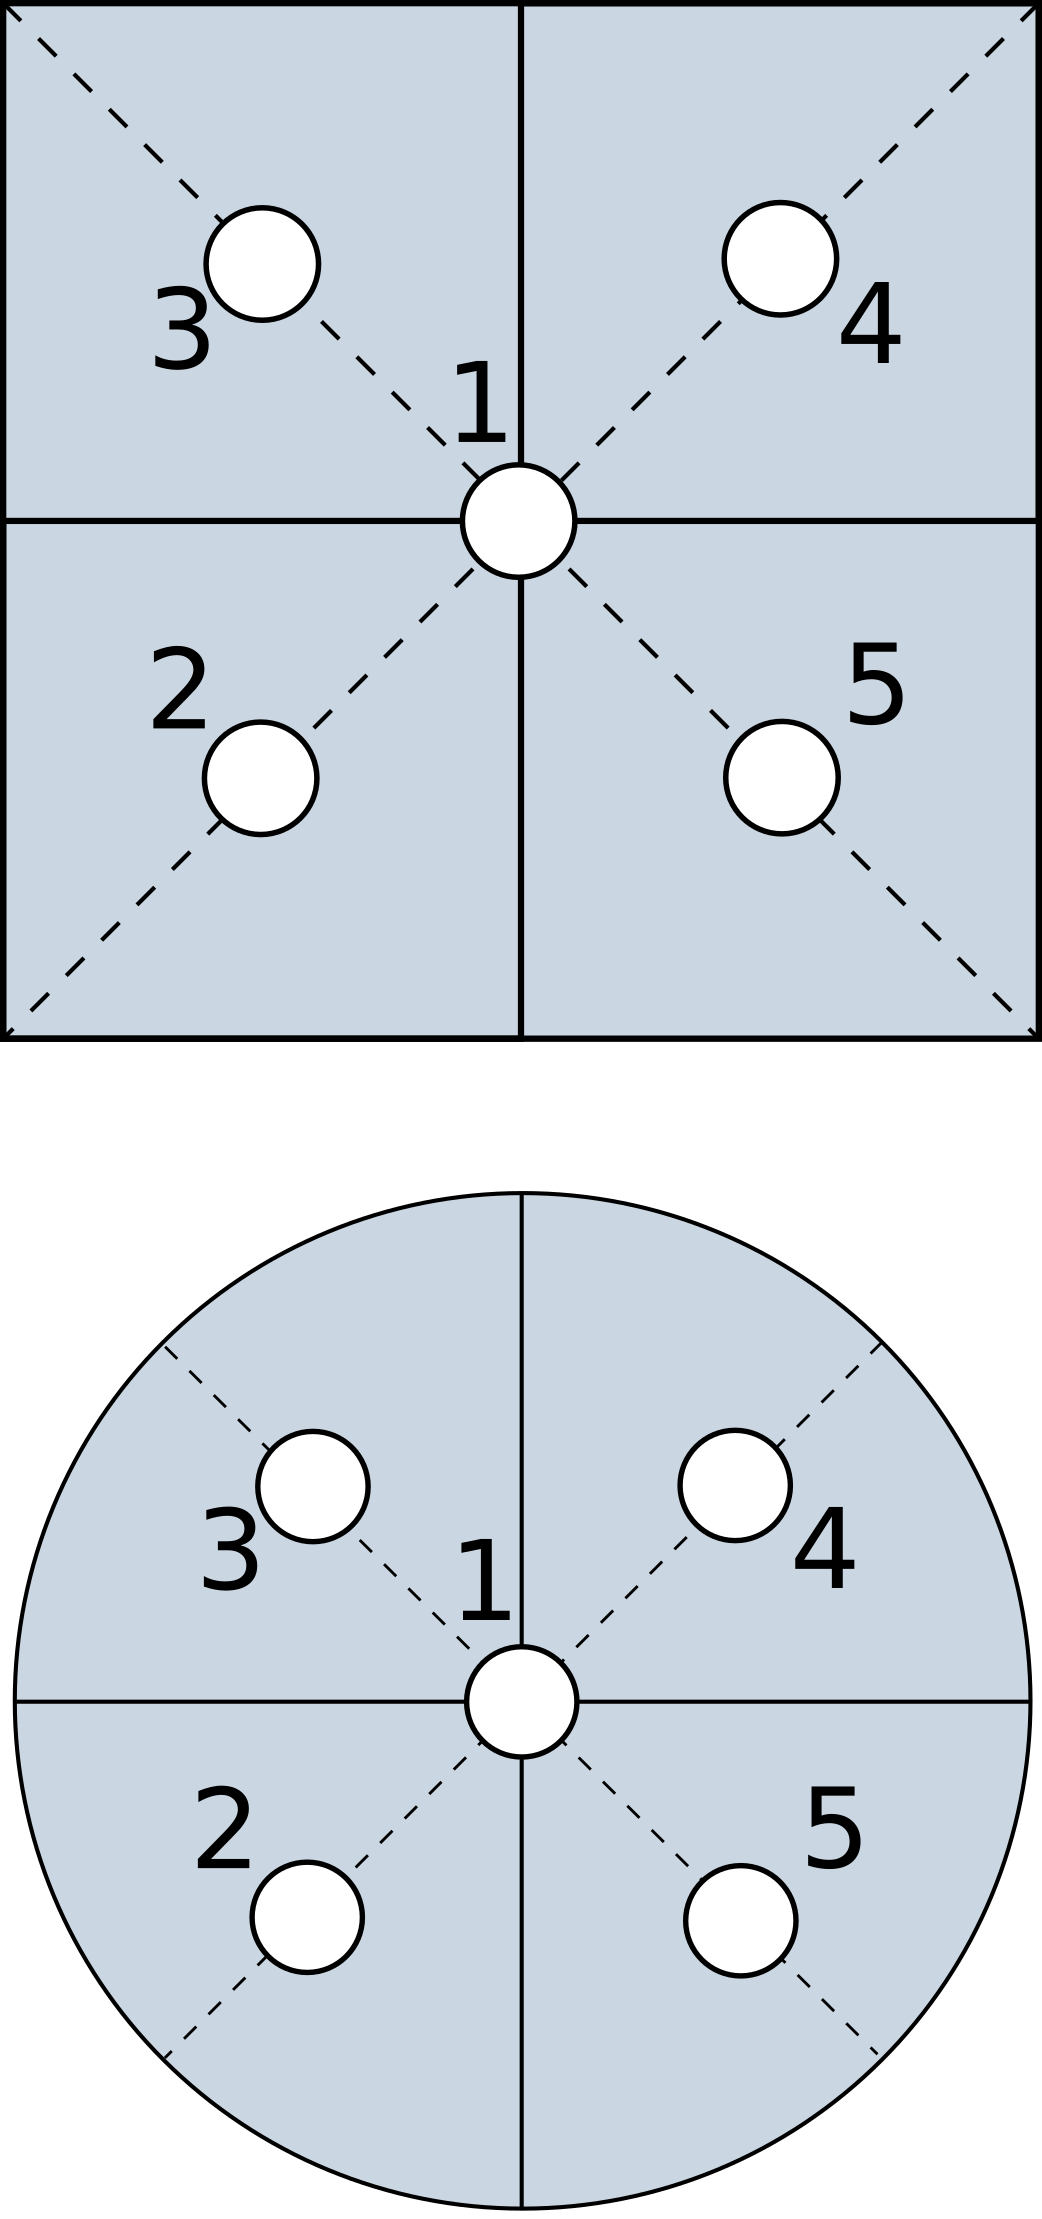
\includegraphics[width = 3cm]{eccen.png}
\end{minipage}
\begin{minipage}{.5\textwidth}

Table: Repeatability test data. Units: [g]

                      Load No. 1 / g   Load No. 2 / g   Load No. 3 / g
-------------------  ---------------  ---------------  ---------------
Ind.1                        0.00999         99.99997        199.99995
Ind.2                        0.00999        100.00001        200.00000
Ind.3                        0.00999         99.99998        199.99998
Ind.4                        0.01000         99.99998        199.99999
Ind.5                        0.01001         99.99997        199.99996
Ind.6                        0.01000         99.99998        199.99996
Ind.7                        0.01001         99.99997        199.99996
Ind.8                        0.01001         99.99996        199.99997
Ind.9                        0.01000         99.99999        199.99995
Ind.10                       0.01001         99.99996        199.99996
.                                                                     
Load                            0.01           100.00           200.00
Standard.deviation           8.8e-06          1.5e-05          1.7e-05


Table: Repeatability test data. Units: [g]

                      Load No. 1 / g   Load No. 2 / g   Load No. 3 / g
-------------------  ---------------  ---------------  ---------------
Ind.1                        0.00999         99.99997        199.99995
Ind.2                        0.00999        100.00001        200.00000
Ind.3                        0.00999         99.99998        199.99998
Ind.4                        0.01000         99.99998        199.99999
Ind.5                        0.01001         99.99997        199.99996
Ind.6                        0.01000         99.99998        199.99996
Ind.7                        0.01001         99.99997        199.99996
Ind.8                        0.01001         99.99996        199.99997
Ind.9                        0.01000         99.99999        199.99995
Ind.10                       0.01001         99.99996        199.99996
.                                                                     
Load                            0.01           100.00           200.00
Standard.deviation           8.8e-06          1.5e-05          1.7e-05
\end{minipage}

\textbackslash end\{document\}

\(\hrulefill\)

\hypertarget{indication-error-test}{%
\subsection{Indication error test}\label{indication-error-test}}

\end{document}
